\documentclass{article}
\usepackage[utf8]{inputenc}
\usepackage{amsmath}
\usepackage{amssymb}
\usepackage{graphicx}
\graphicspath{ {./images} }

\title{Notes on statistical learning}
\author{AvanDavad}

\begin{document}

\maketitle

\section{Linear models and least squares}

On page 12 we have that the residual sum of squares:

\begin{equation}
    \text{RSS}(\beta) = \sum_{i=1}^{N}(y_i-x_i^T\beta)^2 = (\textbf{y} - \textbf{X}\beta)^T(\textbf{y} - \textbf{X}\beta)
\end{equation}

How can we differentiate with respect to $\beta$?

\begin{equation}
    \text{RSS}(\beta) = \textbf{y}^T\textbf{y} - \textbf{y}^T\textbf{X}\beta - \beta^T \textbf{X}^T \textbf{y} + \beta^T \textbf{X}^T \textbf{X} \beta
\end{equation}

We have the following rules for differenciating w.r.t a vector:

\begin{equation}
    \frac{d}{d\textbf{x}}(\textbf{x}^T\textbf{y}) = \frac{d}{d\textbf{x}}(\textbf{y}^T\textbf{x}) = \textbf{y}
\end{equation}

\begin{equation}
    \frac{d}{d\textbf{x}} (\textbf{x}^T \textbf{A} \textbf{x}) = (\textbf{A} + \textbf{A}^T) \textbf{x}
\end{equation}

Using these rules we can differenciate RSS:

\begin{equation}
    \frac{d}{d\beta} \text{RSS}(\beta) = 0 - (\textbf{y}^T \textbf{X})^T - \textbf{X}^T\textbf{y} + (\textbf{X}^T\textbf{X} + (\textbf{X}^T\textbf{X})^T)\beta
\end{equation}

\begin{equation}
    \frac{d}{d\beta} \text{RSS}(\beta) =  -2 \textbf{X}^T\textbf{y} + 2\textbf{X}^T\textbf{X}\beta
\end{equation}

Setting this to zero we get the normal equations:

\begin{equation}
    \textbf{X}^T\textbf{y} = \textbf{X}^T\textbf{X}\beta
\end{equation}

\newpage
\section{Statistical decision theory} \label{linear_fit}

On page 19 we have that

\begin{equation} \label{eq:2_beta}
    \beta = [E(XX^T)]^{-1}E(XY)
\end{equation}

but how exactly do we get this equation? In general, we have the expected prediction error:
\begin{equation}
    \text{EPE}(f) = E(Y-f(X))^2
\end{equation}

And we have that the prediction function is linear:
\begin{equation}
    f(X) = X^T\beta
\end{equation}

We seek a $\beta$ for minimizing the expected prediction error. $X$ and $Y$ are random variables, $X$ being a vector, $Y$ being a scalar. 
\begin{equation}
    \begin{split}
        \frac{d}{d\beta}\text{EPE} = \frac{d}{d\beta} \text{E}((Y-X^T\beta)^2) = \text{E}\left( \frac{d}{d\beta} (Y-X^T\beta)^2\right)\\
        =\text{E} \left( 2(Y - X^T\beta)\cdot (-X) \right) = -2 \text{E} (YX) + 2 \text{E} (X(X^T\beta))\\
         = -2 \text{E} (YX) + 2 \text{E} ((XX^T)\beta) = -2 \text{E} (YX) + 2 (\text{E} (XX^T))\beta
    \end{split}
\end{equation}

We used the fact that the expected value is linear, and that $\beta$ is not random, so we could factor out from the expected value. Setting this to zero we have that:

\begin{equation}
    \text{E} (YX) = \text{E} (XX^T)\beta
\end{equation}

which yields

\begin{equation}
    \hat{\beta} = [\text{E} (XX^T)]^{-1} \text{E} (YX)
\end{equation}

\subsection{application. Simple linear fit.}

Let's see an application for this equation. Let $X=\begin{bmatrix}x\\ 1\end{bmatrix}$, $\beta = \begin{bmatrix}a\\b\end{bmatrix}$.

Now $f(x) = a\cdot x + b$

\begin{equation}
    XY = \begin{bmatrix}x\cdot y \\ y\end{bmatrix}
\end{equation}

\begin{equation}
    XX^T = \begin{bmatrix} x^2 & x \\ x & 1 \end{bmatrix}
\end{equation}

If we have $N$ datapoints $\{(x_1, y_1), (x_2, y_2), ... (x_N, y_N)\}$, we can approximate the expectation values.

\begin{equation}
    \text{E}(XY) \approx \frac 1N \begin{bmatrix}\sum_i x_i\cdot y_i \\ \Sigma_i y_i\end{bmatrix}
\end{equation}

\begin{equation}
    \text{E}(XX^T) \approx \frac 1N \begin{bmatrix} \sum_i x^2_i & \Sigma_i x_i \\ \Sigma_i x_i & N \end{bmatrix}
\end{equation}

Let's denote the followings:

\begin{equation}
    \alpha_X = \sum_i x_i
\end{equation}

\begin{equation}
    \alpha_Y = \sum_i y_i
\end{equation}

\begin{equation}
    \alpha_{XY} = \sum_i x_i y_i
\end{equation}

\begin{equation}
    \alpha_{X^2} = \sum_i x^2_i
\end{equation}

With these notations:

\begin{equation}
    \text{E}(XY) \approx \frac 1N \begin{bmatrix} \alpha_{XY} \\ \alpha_Y \end{bmatrix}
\end{equation}

\begin{equation}
    \text{E}(XX^T) \approx \frac 1N \begin{bmatrix} \alpha_{X^2} & \alpha_X \\ \alpha_X & N \end{bmatrix}
\end{equation}

Inverting $\text{E}(XX^T)$:

\begin{equation}
    [\text{E}(XX^T)]^{-1} \approx \frac{N}{N\alpha_{X^2} - \alpha^2_X} \begin{bmatrix} N & -\alpha_X \\ -\alpha_X & \alpha_{X^2} \end{bmatrix}
\end{equation}

Plug these in to the equation:

\begin{equation}
    \hat{\beta} = [\text{E} (XX^T)]^{-1} \text{E} (YX)
\end{equation}

\begin{equation}
    \hat{\beta} \approx \frac{N}{N\alpha_{X^2} - \alpha^2_X} \begin{bmatrix} N & -\alpha_X \\ -\alpha_X & \alpha_{X^2} \end{bmatrix} \frac 1N \begin{bmatrix} \alpha_{XY} \\ \alpha_Y \end{bmatrix}
\end{equation}

\begin{equation}
    \hat{\beta} \approx \frac{1}{N\alpha_{X^2} - \alpha^2_X} \begin{bmatrix} N \alpha_{XY} -\alpha_X \alpha_Y \\ \alpha_{X^2} \alpha_Y - \alpha_X \alpha_{XY} \end{bmatrix}
\end{equation}


From here we can get $\hat{a}$ and $\hat{b}$, since $\hat{\beta} = \begin{bmatrix} \hat{a} \\ \hat{b} \end{bmatrix}$

\newpage
\section{$\text{E}|Y - c|$ and the median}

On page 20, it asks the question "What happens if we replace the $L_2$ loss function with the $L_1: \text{E}|Y-f(X)|$ ?" Let's investigate this question.

\subsection{discrete case}

We can get rid of the conditional $X=x$, and just ask the question: What $c$ will minimize $\text{E}|Y-c|$? Denote this function with $g$,  so $g(c) = \text{E}|Y-c|$. Let's look at two examples.

Example 1. The random variable $Y$ takes 4 possible values with probabilities $\frac 17$, $\frac 17$, $\frac 37$, $\frac 27$. The figure below shows the probability mass funciton.

\begin{figure}[ht]
 \centering
  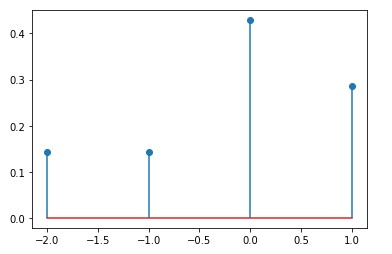
\includegraphics[width=200pt]{images/rnd1}
 \caption{probability mass function of the first example random variable.}
\end{figure}

\begin{figure}[ht]
 \centering
  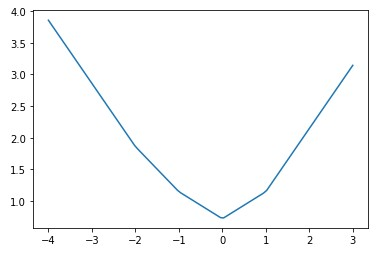
\includegraphics[width=200pt]{images/rnd_func1}
 \caption{$g(c)$ function. The horizontal axis is $c$.}
\end{figure}

Example 2. The random variable $Y$ takes 4 possible values with probabilities 0.1, 0.4, 0.3, 0.2. The figure below shows the probability mass funciton.

\begin{figure}[ht]
 \centering
  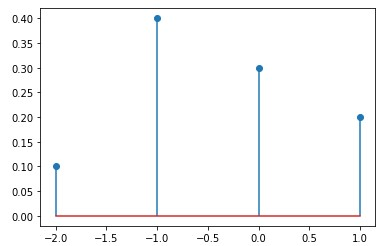
\includegraphics[width=200pt]{images/rnd2}
 \caption{probability mass function of the second example random variable.}
\end{figure}

\begin{figure}[ht]
 \centering
  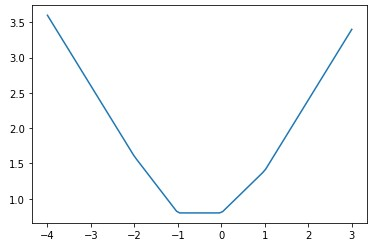
\includegraphics[width=200pt]{images/rnd_func2}
 \caption{$g(c)$ function. The horizontal axis is $c$.}
\end{figure}

We can see that $g(c)$ is a piecewise linear function, and it has minimum, which is a point or a line segment. Let's say we have $Y$ discrete random variable that takes values from $S=\{x_1, x_2, \dots x_n\}$. The values are ordered: $x_1 <  x_2 < ... < x_n$. $Y$ takes these values with corresponding probabilities $p_1$, $p_2$, ..., $p_n$.

Let's calculate the equation of the piecewise linear function. Denote the interval $I_k$ such that $x\in I_k$ if and only if $k$ values from $S$ are smaller than $x$. So $I_0 = (-\infty, x_1]$, $I_1 = [x_1, x_2]$, ..., $I_n = [x_n, \inf)$.

\begin{equation}
    g(c) = \text{E} |Y-c| = \Sigma_{i=1}^{n}p_i \cdot |x_i - c|
\end{equation}

If $c \in I_k$, then

\begin{equation}
    g(c) = \text{E} |Y-c| = \Sigma_{i=1}^{k}p_i \cdot (c - x_i) + \Sigma_{i=k+1}^{n}p_i \cdot (x_i - c)
\end{equation}

\begin{equation}
    g(c) = c\cdot (\Sigma_{i=1}^{k}p_i - \Sigma_{i=k+1}^{n}p_i) + (\Sigma_{i=k+1}^{n}p_i x_i - \Sigma_{i=1}^{k}p_i x_i)
\end{equation}

First we can show that this function is continuous. On one hand ($c\in I_k = [x_k, x_k+1]$):

\begin{equation}
    g_1 = g(x_k) = x_k\cdot (\Sigma_{i=1}^{k}p_i - \Sigma_{i=k+1}^{n}p_i) + (\Sigma_{i=k+1}^{n}p_i x_i - \Sigma_{i=1}^{k}p_i x_i)
\end{equation}

On the other hand we have ($c\in I_{k-1} = [x_{k-1}, x_k]$):

\begin{equation}
    g_2 = g(x_k) = x_k\cdot (\Sigma_{i=1}^{k-1}p_i - \Sigma_{i=k}^{n}p_i) + (\Sigma_{i=k}^{n}p_i x_i - \Sigma_{i=1}^{k-1}p_i x_i)
\end{equation}

\begin{equation}
    g_1 - g_2 = x_k \cdot (p_k + p_k) - p_k x_k - p_k x_k = 0
\end{equation}

Now that we showed that this function is continuous, let's find it's minimum. Since it is piecewise linear, its derivative is piecewise constant. Denote the derivative of $g$ on the interval $I_k$ with $g'(I_k)$.

\begin{equation}
    \begin{split}
        g'(I_k) = -1\\
        g'(I_1)= -1+2p_1\\
        g'(I_2)= -1+2p_1+2p_2\\
        \dots\\
        g'(I_n)= -1+2p_1+...+2p_n=1
    \end{split}
\end{equation}

So the derivative is increasing from $-1$ to $+1$. We can distinguish two possibilities. First, assume that the derivative is never zero. In this case, we have a $k$ where $g'(I_{k-1}) < 0$ but $g'(I_k) > 0$, so the minimum is at $x_k$, the median. The second case is where there is an interval where the derivative is zero. In this case the whole interval is minimum, again, the median.

\subsection{continuous case}

Let's have the following function:

\begin{equation}
    f(x) = \int_{a}^{x}g(x,t)dt
\end{equation}

I state without proof that the derivative of this function is as follows:

\begin{equation}
f'(x) = \int_{a}^{x} \frac{\partial g(x,t)}{\partial x} dt + g(x, x)
\end{equation}

Now we have that

\begin{equation}
    g(c) = \text{E}(|Y-c| | X=x) = \int_{-\infty}^{c}(c-y)f_{Y|X}(y|x)dy + \int_{c}^{\infty}(y-c)f_{Y|X}(y|x)dy
\end{equation}

\begin{equation}
    g'(c) = \int_{-\infty}^{c}f_{Y|X}(y|x)dy + \int_{\infty}^{c}f_{Y|X}(y|x)dy
\end{equation}

Setting this to zero, we get that

\begin{equation}
    \int_{-\infty}^{c}f_{Y|X}(y|x)dy = \int_{c}^{\infty}f_{Y|X}(y|x)dy
\end{equation}

\begin{equation}
    P(Y<c \mid X=x) = P(Y>c \mid X=x)
\end{equation}

Again, this means the minimum is at the median.


\newpage
\section{Local methods in high dimensions}

\subsection{deriving the prediction formula}

On page 24 we see an example of a linear data with noise. At first I was confused how it gets $\hat{y}_0 = x_0^T \beta + \sum_{i=1}^N l_i(x_0)\epsilon_i$, where $l_i(x_0)$ is the $i$th element of $\textbf{X}(\textbf{X}^T\textbf{X})^{-1}x_0$

In this example we make $N$ experiments, storing the $X_i$ values in the rows of $\textbf{X}$, and we have also $\epsilon_i$ (elements of $\vec{\epsilon}$) and $Y_i = X_i^T\beta + \epsilon_i$ for some fixed $\beta$. For approximating $\beta$, we use the result:

\begin{equation}
    \beta = [\text{E} (XX^T)]^{-1} \text{E} (YX)
\end{equation}

in this case it will be an approximation, since we have noise ($\epsilon$).

Calculate first $\text{E} (YX)$:

\begin{equation}
    \text{E} (YX) = \text{E} ((X^T\beta + \epsilon)X) = \text{E} (XX^T)\beta + \text{E} (\epsilon X)
\end{equation}

Substitute this into the approximation of $\beta$:

\begin{equation}
    \begin{split}
        \hat{\beta} = [\text{E} (XX^T)]^{-1} \text{E} (YX)\\
        = [\text{E} (XX^T)]^{-1} (\text{E} (XX^T)\beta + \text{E} (\epsilon X))\\
        = \beta + [\text{E} (XX^T)]^{-1} \text{E} (\epsilon X)
    \end{split}
\end{equation}

We do not know of course the exact expectation values, but we have $N$ data samples (training data). So how could we approximate the expectation values? Use the averages:

\begin{equation}
    \text{E}(\epsilon X)_i \approx \frac{1}{N} \sum_{k=1}^N \textbf{X}_{ki} \epsilon_k \to \text{E} (\epsilon X) \approx \frac{1}{N} \textbf{X}^T \vec{\epsilon}
\end{equation}

similarly,

\begin{equation}
    [\text{E} (XX^T)]^{-1} \approx N \cdot (\textbf{X}^T \textbf{X})^{-1}
\end{equation}

putting these all together, we have:

\begin{equation}
    \hat{y}_0 = x_0^T \hat{\beta} = x_0^T \beta + x_0^T (\textbf{X}^T\textbf{X})^{-1} \textbf{X}^T \vec{\epsilon} = x_0^T \beta + \vec{\epsilon}^T \cdot \textbf{X} (\textbf{X}^T \textbf{X})^{-1} x_0
\end{equation}

and this is the formula that was to be explained.


\subsection{equation (2.47) on page 37}

\begin{equation}
  \begin{split}
    \text{EPE}_k(x_0) = \text{E}\left((Y - \hat{f}_k(x_0))^2 | X=x_0\right)\\
    = \text{E}\left((f(x_0) + \epsilon_0 - \hat{f}_k(x_0))^2\right)
  \end{split}
\end{equation}

The data points are fixed: {$x_1, x_2, \dots, x_N$}. Denote the closest data point to $x_0$ as $x_{(1)}$, the second closest $x_{(2)}$, etc. With this notation, the nearest neighbor estimate for $f(x_0)$:

\begin{equation}
    \hat{f}_k(x_0) = \frac 1k \sum_{l=1}^{k}(f(x_{(l)}) + \epsilon_l)
\end{equation}

In this equation, $f(x_{(l)})$ is fixed, and epsilons are iid random variables.

\begin{equation}
  \begin{split}
    \text{EPE}_k(x_0) = \text{E}\left( \left(f(x_0) + \epsilon_0 - \frac 1k \sum_{l=1}^{k}(f(x_{(l)}) + \epsilon_l)\right)^2\right)\\
    = \text{E}\left( \left[ \left( f(x_0) - \frac 1k \sum_{l=1}^{k}f(x_{(l)})\right) + \left( \epsilon_0 - \frac 1k \sum_{l=1}^{k}\epsilon_l \right) \right]^2 \right)\\
    = \text{E} \left([\hat{F} + \hat{E}]^2\right) = \text{E} \left(\hat{F}^2 + 2\cdot \hat{F} \hat{E} + \hat{E}^2\right) = \hat{F}^2 + 2\hat{F}\cdot\text{E}(\hat{E}) + \text{E}(\hat{E}^2)
  \end{split}
\end{equation}

where $\hat{F}$ is nonrandom, and $\hat{E}$ is random:

\begin{equation}
  \begin{split}
    \hat{F} \equiv f(x_0) - \frac 1k \sum_{l=1}^{k}f(x_{(l)}),\\
    \hat{E} \equiv \epsilon_0 - \frac 1k \sum_{l=1}^{k}\epsilon_l
  \end{split}
\end{equation}

Let's calculate the expectation of $\hat{E}$:

\begin{equation}
    \text{E} (\hat{E}) = \text{E} \left( \epsilon_0 - \frac 1k \sum_{l=1}^{k}\epsilon_l \right) = \text{E} (\epsilon_0) - \frac 1k \sum_{l=1}^{k}\text{E} (\epsilon_l) = 0 - \frac 1k \sum_{l=1}^{k}0 = 0
\end{equation}

The expectation of $\hat{E}^2$:

\begin{equation}
    \text{E} (\hat{E}^2) = \text{E} \left( \epsilon_0 - \frac 1k \sum_{l=1}^{k}\epsilon_l \right)^2 = \text{E} \left( \epsilon_0^2 + \sum_{l=1}^{k}\frac{\epsilon_l^2}{k^2} + CrossProducts \right)
\end{equation}

The expectation of the cross products are zero, since epsilons are independent, so $\text{E}(\epsilon_i \epsilon_j) = \text{E} \epsilon_i \cdot \text{E} \epsilon_j = 0\cdot 0 = 0$

\begin{equation}
  \begin{split}
    \text{E} (\hat{E}^2) = \text{E} \left( \epsilon_0^2 + \sum_{l=1}^{k}\frac{\epsilon_l^2}{k^2} \right) = \text{E} \epsilon_0^2 + \sum_{l=1}^{k}\frac{\text{E}\epsilon_l^2}{k^2}\\
    = \sigma^2 + \sum_{l=1}^{k}\frac{\sigma^2}{k^2} = \sigma^2 + \frac{\sigma^2}{k}
  \end{split}
\end{equation}

We used the fact that the error has zero mean, so the variance is $\sigma^2 = \text{Var}(\epsilon) = \text{E}(\epsilon^2) - (\text{E}\epsilon)^2 = \text{E}(\epsilon^2)$. So the final form is:

\begin{equation}
  \begin{split}
    \text{E}_k(x_0) = \hat{F}^2 + 2\hat{F}\cdot\text{E}(\hat{E}) + \text{E}(\hat{E}^2) = \hat{F}^2 + \text{E}(\hat{E}^2)\\
    = \left( f(x_0) - \frac 1k \sum_{l=1}^{k}f(x_{(l)}) \right)^2 + \sigma^2 + \frac{\sigma^2}{k}
  \end{split}
\end{equation}

\section{Solutions for the Exercises of chapter 2}

\subsection{Ex. 2.2}

We have $X \in \mathbb{R}^p$ continuous and $G$ discrete random variables. Assume we have $K$ classes. Each class has its own distribution, let's say that class $g$ has a pdf $f_{g}(x)$ ($x \in \mathbb{R}^p$). When generating points, we first choose a class with associated probabilities $p_1, p_2, \dots, p_K$ ($\sum p_i = 1$). When we have chosen the class, we generate a point with the appropriate distribution.

The Bayes classifier classifies each point $x$ to the most probable class. So let's calculate the probability of class $g$, given the point. It should be noted that when I write $\text{P}(x)$, I mean "the probability that the chosen point is in the infinitesimal neighborhood of $x$". So I should write $\text{P}(X \in b_{dx}(x))$, i.e., the probability that $X$ is in the $dx$-volume ball around $x$. If the pdf was $f(x)$, this probability is $f(x)dx$. But instead, I'll write $\text{P}(x) = f(x)$. Likewise, when I write $\text{P}(g)$, I mean $\text{P}(G=g)$.

\begin{equation}
    \text{P}(g|x) = \frac{\text{P}(g \cap x)}{\text{P}(x)} = \frac{\text{P}(g \cap x)}{\text{P}(x)} = \frac{\text{P}(x | g) \text{P}(g)}{\sum_{g'}\text{P}(x|g') \text{P}(g')}
\end{equation}

The denominator is a normalizing constant, so the chosen class, for which $\text{P}(g|x)$ is maximum:

\begin{equation}
    \hat{g}(x) = max_{g} \text{P} (x|g) \text{P}(g)
\end{equation}

\subsection{Ex. 2.3}

Given a unit ball in $p$-dimension. We sample $N$ data points from it uniformly. Let $X$ be the distance from the origin. The pdf must be proportional to $x^{p-1}$, and integrating it from 0 to 1 gives 1, thus the pdf:

\begin{equation}
    f(x) = p\cdot x^{p-1}
\end{equation}

The probability that a random sample is at least $x$ distant from the origin is:

\begin{equation}
    \text{P}(X > x) = \int_{x}^{1} f(x)dx = 1 - x^p
\end{equation}

The probability that all $N$ sample points are further from origin as $x$:

\begin{equation}
    \text{P}(X_1 > x \cap X_2 > x \cap \dots \cap X_N > x) = \left( 1 - x^p \right)^N
\end{equation}

We seek and $x$ for that this probability is a half (that will give us the median):

\begin{equation}
  \begin{split}
    \left( 1 - x^p \right)^N = \frac 12\\
    1 - x^p = \left(\frac 12\right)^{1/N}\\
    \left[1 - \left(\frac 12\right)^{1/N}\right]^{1/p} = x
  \end{split}
\end{equation}


\subsection{Ex. 2.4}

If we choose $a$ as the first unit base vector ($a=[1,0,0,\dots,0]^T$), then $a^T \cdot x_i$ is the first coordinate of $x_i$. It is by definition (standard) normally distributed. Since the distribution is spherically symmetric, we can choose any direction $a$, $a^T \cdot x_i$ remains standard normal.

I created an experiment on this. Created 1000 sample points in $p$ dimension, and rotated them into the first 2 dimension, so that we can visualize the distances. On the first image below we can see that the points get further and further away from the origin as the dimension increases.

\begin{figure}[ht]
 \centering
  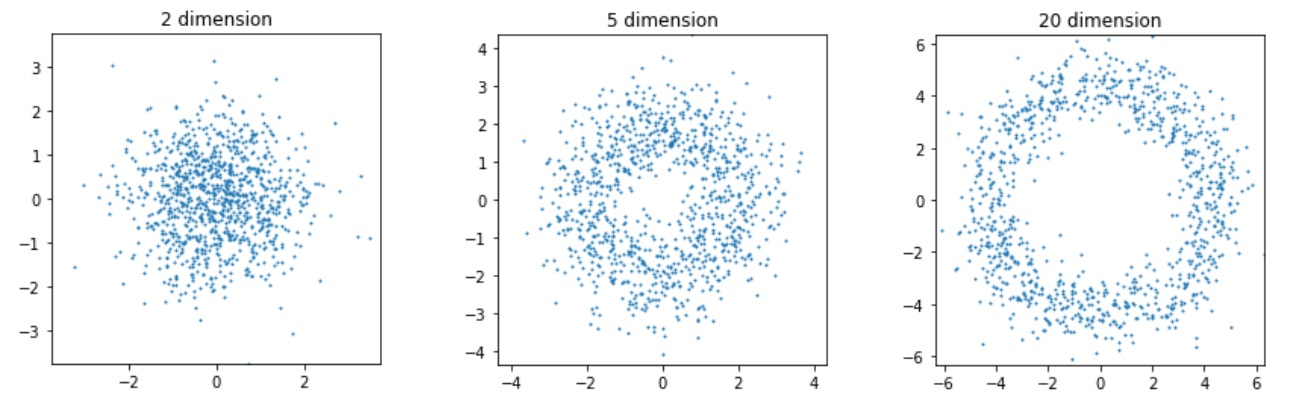
\includegraphics[width=200pt]{images/ex2_2_origin.jpg}
 \caption{The sample points get further from the origin as we increase the dimension.}
\end{figure}

But this doesn't mean the points are close from each other. In the following experiment I took the random sample points, chose one of them and set it as the new origin. We can see that still the points are far from a random sample point as we increase the dimension.

\begin{figure}[ht]
 \centering
  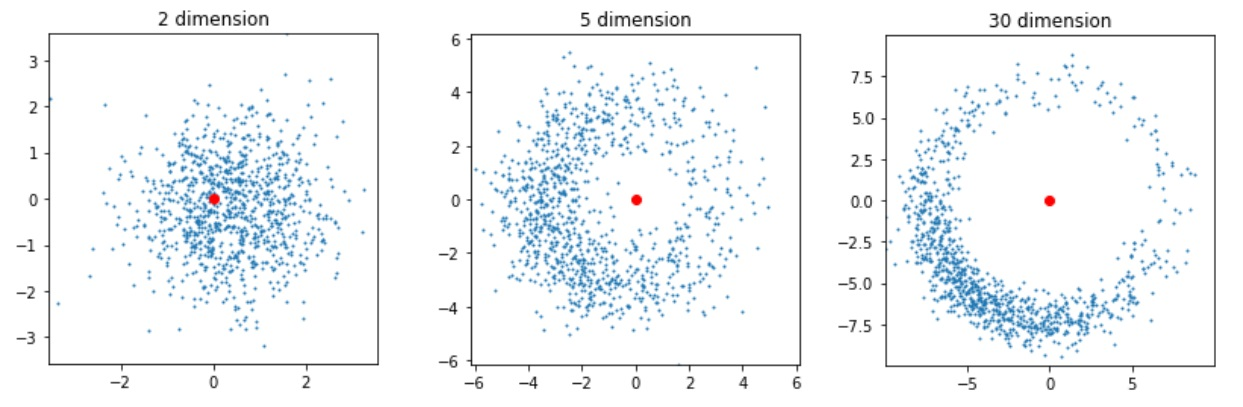
\includegraphics[width=200pt]{images/ex_2_2_sample.jpg}
 \caption{The points get further and further from each other (red dot is a randomly selected sample point) as we increase the dimension.}
\end{figure}

\subsection{Ex. 2.5}

\subsubsection{equation (2.27) on page 26}

I won't use indices at the expectation sign, it always confuses me. So this is the expected prediction error:

\begin{equation}
    \text{EPE}(x_0) = \text{E}(y_0 - \hat{y}_0)^{2}
\end{equation}

Recall, that $y_0 = x_0^T \beta + \epsilon$ is a random variable, since $\epsilon \sim N(0,\sigma^2)$. This is the label (the ground truth) for $x_0$. The prediction that we make for $x_0$ is $\hat{y_0} = x_0^T \beta + \vec{\epsilon}^T \cdot \textbf{X} (\textbf{X}^T \textbf{X})^{-1} x_0$. $x_0$ is a $p$-vector, $\beta$ is a $p$-vector, $\vec{\epsilon}$ is an $n$-vector, and $\mathbf{X}$ is a $n$ by $p$ matrix (each row is a training sample vector). $\hat{y}_0 = x_0^T \beta + \vec{\epsilon}^T \cdot \textbf{Z}^T x_0$. Here I introduced the $p$ by $n$ matrix $\textbf{Z}$:

\begin{equation}
    \textbf{Z} \equiv (\textbf{X}^T \textbf{X})^{-1} \textbf{X}^T
\end{equation}

In the expression of $\hat{y}_0$, $\vec{\epsilon}$ and $\textbf{Z}$ are the only random variables. The elements of $\vec{\epsilon}$ are iid RVs. $\vec{\epsilon}$ and $\textbf{Z}$ are independent. Let's calculate the expectation values of $y_0$ and $\hat{y}_0$:

\begin{equation}
    \text{E}(y_0) = \text{E} (x_0^T \beta + \epsilon) = x_0 ^ T \beta
\end{equation}

\begin{equation}
  \begin{split}
    \text{E}(\hat{y}_0) = \text{E} (x_0^T \beta + \vec{\epsilon}^T \cdot \textbf{Z}^T x_0)\\
    = x_0^T \beta + \text{E}(\vec{\epsilon}^T \cdot \textbf{Z}^T x_0) \\
    = x_0^T \beta + \text{E}(\vec{\epsilon}^T) \text{E} (\textbf{Z}^T x_0) \\
    = x_0^T \beta + \vec{0}^T \cdot \text{E} (\textbf{Z}^T x_0) \\
    = x_0^T \beta
  \end{split}
\end{equation}

Here I used that $\vec{\epsilon}$ and $\textbf{Z}$ are independent, so the expectation value of their product is the product of their expectations. For simplicity, denote $\mu \equiv \text{E}(y_0) = \text{E}(\hat{y}_0) = x_0^T \beta$. The expected prediction error:

\begin{equation}
  \begin{split}
    \text{EPE}(x_0) = \text{E} (y_0 - \mu + \mu - \hat{y}_0)^2 \\
    = \text{E} (y_0 - \mu) ^ 2 - 2 \cdot \text{E} ((y_0 - \mu)(\hat{y}_0 - \mu)) + \text{E} (\hat{y}_0 - \mu)^2\\
    = \text{E} (y_0 - \mu) ^ 2 + 0 + \text{E} (\hat{y}_0 - \mu) ^ 2\\
    = \text{Var}(y_0) + \text{Var}(\hat{y}_0)
  \end{split}
\end{equation}

Note that $y_0$ and $\hat{y}_0$ are independent. The epsilon in $y_0$ is a scalar and is nothing to do with the vector epsilon in $\hat{y}_0$. This is why $\text{E} ((y_0 - \mu)(\hat{y}_0 - \mu))$ is zero. Now let's derive the variances:

\begin{equation}
    \text{Var}(y_0) = \text{Var}(\mu + \epsilon) = \text{Var}(\epsilon) = \sigma ^2
\end{equation}

This was the easy part. It is much more difficult to get the variance for $\hat{y}_0$. We know that if $a$ is a constant scalar, and $X$ is a scalar random variable, then

\begin{equation}
    \text{Var}(aX) = a^2 \cdot \text{Var}(X)
\end{equation}

Okay, but what if $a$ is a vector, just as $X$, and we take the inner product $a^T\cdot X$? What is the variance $\text{Var}(a^T\cdot X)$?

\begin{equation}
\begin{split}
    \text{Var}(a^T\cdot X) = \text{Var}(a_1 \cdot X_1 + a_2 \cdot X_2 + \dots + a_n \cdot X_n)\\
    = \text{E} \left( \sum_{i} a_i \cdot (X_i - \text{E} X_i)\right)^2\\
    = \text{E} \left( \sum_{i,j} a_i  \cdot (X_i - \text{E} X_i) \cdot a_j \cdot (X_j - \text{E} X_j)\right)\\
    = \sum_{i,j} a_i \cdot a_j \cdot \text{E} \left( (X_i - \text{E} X_i) \cdot (X_j - \text{E} X_j) \right)\\
    = \sum_{i,j} a_i \cdot a_j \cdot \text{Cov}(X_i, X_j)\\
    = a^T \cdot \text{Cov}(X,X) \cdot a = a^T \cdot \Sigma \cdot a
\end{split}
\end{equation}

Here $\Sigma \equiv \text{Cov}(X,X)$ is the covariance matrix, $\text{Cov}(X,X)_{i,j} = \text{Cov}(X_i, X_j)$. Let's state our finding again. $a$ is a constant vector, $X$ is a random vector (same dimension), then:

\begin{equation}
    \text{Var}(a^T \cdot X) = a^T \cdot \text{Cov}(X,X) \cdot a
\end{equation}

Furthermore, we can write $\text{Cov}(X,X) = \text{E} ((X-\text{E}X)\cdot (X-\text{E}X)^T) = \text{E}(X\cdot X^T) - (\text{E}X) (\text{E}X^T)$. Now we can apply this to derive the variance of $\hat{y}_0$:

\begin{equation} \label{eq:1}
  \begin{split}
    \text{Var}(\hat{y}_0) = \text{Var}(\mu + x_0^T \cdot \textbf{Z} \cdot \vec{\epsilon}) = \text{Var} (x_0^T \cdot \textbf{Z} \cdot \vec{\epsilon})\\
     = x_0^T \cdot \text{Cov}(\textbf{Z} \cdot \vec{\epsilon}, \textbf{Z} \cdot \vec{\epsilon}) \cdot x_0\\
     = x_0^T \cdot \left( \text{E}(\textbf{Z} \vec{\epsilon} \cdot \vec{\epsilon}^T \textbf{Z}^T) - \text{E}(\textbf{Z}\vec{\epsilon}) \cdot \text{E} (\vec{\epsilon}^T \textbf{Z}^T) \right) \cdot x_0\\
     = x_0^T \cdot \text{E}(\textbf{Z} \vec{\epsilon} \cdot \vec{\epsilon}^T \textbf{Z}^T)  \cdot x_0
  \end{split}
\end{equation}

Here we used the fact that $\textbf{Z}$ and $\vec{\epsilon}$ are independent, so $\text{E}(\textbf{Z} \vec{\epsilon}) = \text{E}\textbf{Z} \cdot \text{E} \vec{\epsilon} = \text{E}\textbf{Z} \cdot \vec{0} = \vec{0}$, and $\vec{0} \cdot \vec{0}^T = \textbf{0}$, zero matrix.

\begin{equation}
  \begin{split}
    \left( \textbf{Z} \vec{\epsilon} \cdot \vec{\epsilon}^T \textbf{Z}^T \right)_{i,j} = \sum_{k,l} (\textbf{Z})_{i,k} \cdot (\vec{\epsilon} \vec{\epsilon}^T)_{k,l} \cdot (\textbf{Z}^T)_{l,j}\\
    \to \text{E} \left( \textbf{Z} \vec{\epsilon} \cdot \vec{\epsilon}^T \textbf{Z}^T \right)_{i,j} = \sum_{k,l} \text{E} \left( Z_{i,k} \cdot \epsilon_k \cdot \epsilon_l \cdot Z_{j,l} \right)\\
    = \sum_{k,l} \text{E} \left( Z_{i,k} \cdot Z_{j,l} \right) \cdot \text{E} \left( \epsilon_k \cdot \epsilon_l \right) = \sum_{k,l} \text{E} \left( Z_{i,k} \cdot Z_{j,l} \right) \cdot \sigma^2 \delta_{k,l}\\
    = \sigma^2 \cdot \sum_{k} \text{E} \left( Z_{i,k} \cdot Z_{j,k} \right) = \sigma^2 \cdot \text{E} \sum_{k} \left( Z_{i,k} \cdot Z_{j,k} \right) = \sigma^2 \cdot \text{E} (\textbf{Z} \textbf{Z}^T)_{i,j}\\
    \to \text{E}(\textbf{Z} \vec{\epsilon} \cdot \vec{\epsilon}^T \textbf{Z}^T) = \sigma^2 \cdot \text{E} (\textbf{Z} \textbf{Z}^T)
  \end{split}
\end{equation}

Substituting this into (\ref{eq:1}):

\begin{equation}
    \text{Var}(\hat{y}_0) = x_0^T \cdot \sigma^2 \text{E} (\textbf{Z} \textbf{Z}^T) \cdot x_0
\end{equation}

\begin{equation}
    \text{E}(\textbf{Z} \textbf{Z}^T) = \text{E} \left( (\textbf{X}^T \textbf{X})^{-1} \textbf{X}^T \textbf{X} (\textbf{X}^T \textbf{X})^{-1} \right) = \text{E} \left( (\textbf{X}^T \textbf{X})^{-1} \right)
\end{equation}

Putting it all together:

\begin{equation}
    \text{EPE}(x_0) = \text{Var} (y_0) + \text{Var} (\hat{y}_0) = \sigma^2 + \sigma^2 \cdot x_0^T \cdot \text{E} \left( (\textbf{X}^T \textbf{X})^{-1} \right) \cdot x_0
\end{equation}

And this is what we wanted to derive.

\subsubsection{equation (2.28) on page 26}

\begin{equation}
    \text{E} \left( x^T_0 \text{Cov}(X)^{-1}x_0 \right) = \text{E} \sum_{i,j} x_{0,i} \text{Cov}(X)^{-1}_{i,j} x_{0,j}
\end{equation}

Assuming that $x_0 \sim X$, i.e., $x_0$ (the test point) has the same distribution as $X$ (the training data), and the expectation of it is the zero vector, $\text{Cov}(x_0) = \text{Cov}(X) = \text{E} (x_0 x^T_0)$.

\begin{equation}
  \begin{split}
    \text{E} \sum_{i,j} x_{0,i} \text{Cov}(X)^{-1}_{i,j} x_{0,j} = \text{E} \sum_{i,j} \text{Cov}(X)^{-1}_{i,j} \text{Cov}(x_0)_{i,j}\\
    = \text{E} \sum_{i,j} \text{Cov}(X)^{-1}_{i,j} \text{Cov}(X)_{i,j} = \text{E} \sum_{i} \left( \sum_{j} \text{Cov}(X)^{-1}_{i,j} \text{Cov}(X)_{j,i} \right)\\
    = \text{E} \sum_{i} [\text{Cov}(X)^{-1} \text{Cov}(X)]_{i,i} = \text{E} \left( \text{Trace} (\text{Cov}(X)^{-1} \text{Cov}(X)) \right) \\
    = \text{E} \left( \text{Trace} I_{pxp} \right) = p
  \end{split}
\end{equation}


\subsection{Ex. 2.6}

Assume that we have $n$ identical inputs $x_1 = x_2 = \dots = x_n \equiv x$ with outputs $y_1$, $y_2$, $\dots$, $y_n$. The least squares formula:

\begin{equation} \label{eq:ex2.6.1}
    RSS(\theta) = \sum_{i=1}^{n} (y_i - f_{\theta}(x))^2
\end{equation}

The weighted least squares formula:

\begin{equation} \label{eq:eq2.6.2}
    RSS_w(\theta) = n\cdot \left(\frac{\sum_{i=1}^{n}y_i}{n} - f_{\theta}(x)\right)^2
\end{equation}

I claim that the two expressions differ by a constant term that doesn't depend on $\theta$, so both expressions lead to the same solution. This naturally extends to the case when we have groups of equal inputs.

Expanding $RSS$:

\begin{equation}
    RSS(\theta) = \sum_{i=1}^{n}y_i^2 - 2 f_{\theta}(x) \sum_{i=1}^{n} y_i + f_{\theta}^2(x)
\end{equation}

Expanding $RSS_w$:

\begin{equation}
    RSS_w(\theta) = \frac{\left( \sum_{i=1}^{n} y_i \right)^2}{n} - 2 f_{\theta}(x) \sum_{i=1}^{n} y_i + f_{\theta}^2(x)
\end{equation}

So the difference of the 2 expressions is a constant that doesn't depend on $\theta$. So when we derive wrt $\theta$, we get the same formulae.

Whenever we have observations with identical values $x$, we can always refactor the $RSS$ for the groups according to (\ref{eq:ex2.6.1}) $\to$ (\ref{eq:eq2.6.2}).

\subsection{Ex. 2.7}

Our estimator according to the problem statement:

\begin{equation}
    \hat{f}(x_0) = \sum_{i=1}^{N}l_i(x_0;\mathcal{X})y_i
\end{equation}

a) For kNN, the weights are:


\begin{equation}
    l_i(x_0;\mathcal{X}) = \frac{1}{k} \delta(x_i \in \text{kNN}(x_0))
\end{equation}

where $\delta(x_i \in \text{kNN}(x_0))$ is $1$ if $x_i$ is in the set of k-nearest neighbors of $x_0$, and $0$ otherwise. So in this case we average the $y$s of the k-nearest neighbors of $x_0$.

For linear regression we have

\begin{equation}
    \hat{f}(x_0) = x_0^T \beta
\end{equation}

Where $\beta$ comes from  the following equation (see Section \ref{linear_fit}):

\begin{equation}
    \beta = \text{E}(XX^T)^{-1}\text{E}(XY)
\end{equation}

Now let's calculate this expression. We estimate the expectation values with averages.

\begin{equation}
    \begin{split}
        \text{E}(XX^T)^{-1} \approx \left( \frac{1}{N}\sum_{j=1}^{N}x_j x^T_j\right)^{-1}\\
        \text{E}(XY) \approx \frac{1}{N}\sum_{i=1}^{N}x_i y_i\\
    \end{split}
\end{equation}

With these, we can formulate $\hat{f}(x_0)$ as follows:

\begin{equation}
  \begin{split}
    \hat{f}(x_0) = x^T_0 \left( \frac{1}{N}\sum_{j=1}^{N}x_j x^T_j\right)^{-1} \cdot \frac{1}{N}\sum_{i=1}^{N}x_i y_i\\
    = \sum_{i=1}^{N} x^T_0 \left( \sum_{j=1}^{N} x_j x^T_j \right)^{-1} x_i y_i \\
    \equiv \sum_{i=1}^{N} l_i(x_0;\mathcal{X}) y_i
  \end{split}
\end{equation}

From this we get the weights:

\begin{equation}
    l_i(x_0; \mathcal{X}) = x^T_0 \left( \sum_{j=1}^{N} x_j x^T_j \right)^{-1} x_i
\end{equation}

\end{document}